\documentclass{scrartcl}

% neccesarry for style
\usepackage[english]{babel}
\usepackage[utf8]{inputenc}
\usepackage[T1]{fontenc}
\usepackage{lmodern}

% tools for text
\usepackage{csquotes}
\usepackage{url}
\usepackage{hyperref}

% graphics
\usepackage{graphicx}
\usepackage{xcolor}
\usepackage{tikz}

% maths
\usepackage{amsmath,amssymb,amstext,amsthm}

% programming
\usepackage{listings}

\usepackage{wasysym} %lightning

\input{required/settings.tex}
\input{required/commands.tex}

\renewcommand{\labelenumi}{\alph{enumi})}
\begin{document}
	\begin{center}
		\LARGE
		Information Integration -- Exercise 6 -- Gabriel Glaser
	\end{center}
	
	\section*{Task 1: LaV and the Bucket Algorithm}
	\begin{center}
		\fbox{
			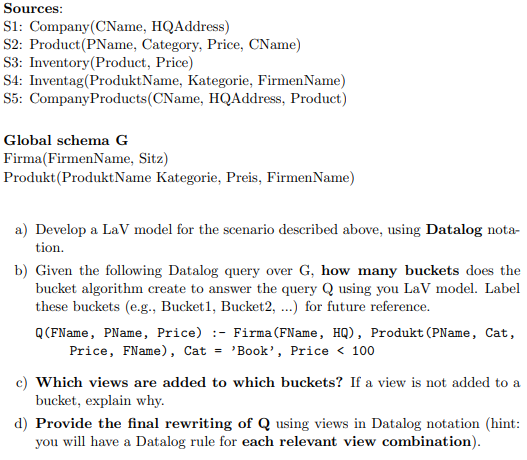
\includegraphics[width=0.7\textwidth]{figures/t1.PNG}
		}
	\end{center}
	\begin{enumerate}
		\item\phantom{phantom}
		\begin{itemize}
			\item S1:
			\begin{center}
				\fbox{
					\begin{tabular}{l}
						S1(FirmenName, Sitz) :--\\
						\hspace{0.5cm}Firma(FirmenName, Sitz)
					\end{tabular}
				}
			\end{center}
			S1 exactly the same than relation \enquote{Firma}.
			
			\item S2:
			\begin{center}
				\fbox{
					\begin{tabular}{l}
						S2(ProduktName, Kategorie, Preis, FirmenName) :--\\
						\hspace{0.5cm}Produkt(ProduktName, Kategorie, Preis, FirmenName)
					\end{tabular}
				}
			\end{center}
			S2 exactly the same than relation \enquote{Produkt}.
			
			\item S3:
			\begin{center}
				\fbox{
					\begin{tabular}{l}
						S3(ProduktName, Preis) :--\\
						\hspace{0.5cm}Produkt(ProduktName, Kategorie, Preis, FirmenName)\\
					\end{tabular}
				}
			\end{center}
			\textit{Assumption}: \enquote{ProduktName} and \enquote{PName} are the primary keys for their respective relation (Produkt / Product).
			Thus, they can be used as a foreign key to reference a product.
			
			\item S4:
			\begin{center}
				\fbox{
					\begin{tabular}{l}
						S4(ProduktName, Kategorie, FirmenName) :--\\
						\hspace{0.5cm}Produkt(ProduktName, Kategorie, Preis, FirmenName)
					\end{tabular}
				}
			\end{center}
			Basically S4 is the same table than \enquote{Produkt} but doesn't include the attribute \enquote{Preis}.
			
			\item S5:
			\begin{center}
				\fbox{
					\begin{tabular}{l}
						S5(FirmenName, Sitz, ProduktName) :--\\
						\hspace{0.5cm}Firma(FirmenName, Sitz),\\
						\hspace{0.5cm}Produkt(ProduktName, Kategorie, Preis, FirmenName)
					\end{tabular}
				}
			\end{center}
			Join both global schema tables according to \enquote{FirmenName} to get S5.
		\end{itemize}
		
		\item
		Given query $Q$ over global schema $G$ needs two buckets, because $Q$ has two sub-goals.
		The bucket for \textit{Firma} is called \enquote{Bucket$_\text{Firma}$} and the bucket for \textit{Produkt} is called \enquote{Bucket$_\text{Produkt}$}
		
		\item\phantom{phantom}
		\begin{itemize}
			\item Bucket$_\text{Firma}$ corresponding to Firma(FName, HQ), all sub-goals of all views:
			\begin{itemize}
				\item \textit{S1.Firma(FirmenName, Sitz)} $\checked$
				\item \textit{S2.Produkt(ProduktName, Kategorie, Preis, FirmenName)} $X$ (Doesn't contain HQ)
				\item \textit{S3.Produkt(ProduktName, Kategorie, Preis, FirmenName)} $X$ (Doesn't contain HQ)
				\item \textit{S4.Produkt(ProduktName, Kategorie, Preis, FirmenName)} $X$ (Doesn't contain HQ)
				\item \textit{S5.Firma(FirmenName, Sitz)} $\checked$
				\item \textit{S5.Produkt(ProduktName, Kategorie, Preis, FirmenName)} $X$ (Doesn't contain HQ)
			\end{itemize}
			$\Rightarrow$ S1, S5
			
			\item Bucket$_\text{Produkt}$ corresponding to Produkt(PName, Cat, Price, FName), all sub-goals of all views:
			\begin{itemize}
				\item \textit{S1.Firma(FirmenName, Sitz)} $X$ (Doesn't contain needed attributes)
				\item \textit{S2.Produkt(ProduktName, Kategorie, Preis, FirmenName)} $\checked$
				\item \textit{S3.Produkt(ProduktName, Kategorie, Preis, FirmenName)} $X$ (Price and Cat not preserved by S3)
				\item \textit{S4.Produkt(ProduktName, Kategorie, Preis, FirmenName)} $X$ (Price not preserved by S4)
				\item \textit{S5.Firma(FirmenName, Sitz)} $X$ (Doesn't contain PName, Cat, Price)
				\item \textit{S5.Produkt(ProduktName, Kategorie, Preis, FirmenName)} $X$ (Price and Category not preserved by S4)
			\end{itemize}
			$\Rightarrow$ S2
		\end{itemize}
		
		\item Datalog queries (not optimized):
		\begin{itemize}
			\item S1, S2:
			\begin{center}
				\fbox{
					\begin{tabular}{l}
						Q(FirmenName, ProduktName, Preis) :--\\
						\hspace{0.5cm}S1(FirmenName, Sitz),\\
						\hspace{0.5cm}S2(ProduktName, Kategorie, Preis, FirmenName)
					\end{tabular}
				}
			\end{center}
			\item S5, S2:
			\begin{center}
				\fbox{
					\begin{tabular}{l}
						Q(FirmenName, ProduktName, Preis) :--\\
						\hspace{0.5cm}S5(FirmenName, Sitz, ProduktName),\\
						\hspace{0.5cm}S2(ProduktName, Kategorie, Preis, FirmenName)
					\end{tabular}
				}
			\end{center}
		\end{itemize}
	\end{enumerate}
	
	\section*{Task2: Bucket Algorithm (Sample exam question)}
	\begin{center}
		\fbox{
			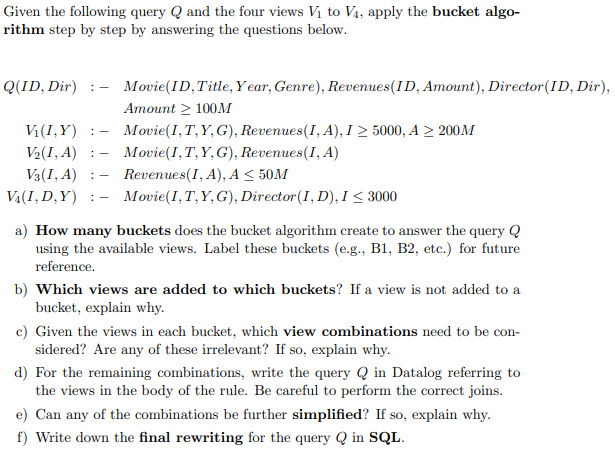
\includegraphics[width=0.7\textwidth]{figures/t2.PNG}
		}
	\end{center}
	\begin{enumerate}
		\item The bucket algorithm needs \textit{three} buckets, $B_\text{Movie}$, $B_\text{Revenues}$ and $B_\text{Director}$.
		
		\item\phantom{phantom}
		\begin{itemize}
			\item $B_\text{Movie}$ with Movie(ID, Title, Year, Genre):
			% 1. relation + variables match
			% 2. Predicates / Integrity Constraints do not contradict
			% 3. q(...x...)  with subplan/relation(...x...) => view for subplan = v(...x...)
			\begin{itemize}
				\item V1: 1. Movie(ID, Title, Year, Genre) = Movie(I, T, Y, G), 2. I $\geq5000$ doesn't contradict, 3. Variables of $Q$ which are in $Q$.Movie are also in V1.
				\item V2: 1. Movie(ID, Title, Year, Genre) = Movie(I, T, Y, G), 2. No contradictions, 3. Variables of $Q$ which are in $Q$.Movie are also in V2.
				\item not V3 (wrong relation)
				\item V4: 1. Movie(ID, Title, Year, Genre) = Movie(I, T, Y, G), 2. I $\leq3000$ doesn't contradict, 3. Variables of $Q$ which are in $Q$.Movie are also in V1.
			\end{itemize}
			$\Rightarrow$ V1, V2, V4
			
			\item $B_\text{Revenues}$ with Revenues(ID, Amount):
			\begin{itemize}
				\item V1: 1. Revenues(ID, Amount) = Revenues(I, A), 2. predicates don't contradict, 3. Variables of $Q$ which are in $Q$.Revenues (i.e., ID) are also in V2 (i.e., I).
				\item V2: $\checked$
				\item not V3, because predicates contradict.
				\item not V4 (wrong relation)
			\end{itemize}
			$\Rightarrow$ V1, V2
			
			\item $B_\text{Director}$ with Director(ID, Dir):
			\begin{itemize}
				\item not V1 (wrong relation)
				\item not V2 (wrong relation)
				\item not V3 (wrong relation)
				\item V4 $\checked$
			\end{itemize}
			$\Rightarrow$ V4
		\end{itemize}
		
		\item Combinations:
		\begin{itemize}
			\item V1, V1, V4: I $\leq 3000$ $\wedge$ I $\geq 5000$ $X$ (V1 contradicts with V4)
			\item V1, V2, V4: $X$
			\item V2, V1, V4: $X$
			\item V2, V2, V4:
			\item V4, V1, V4: $X$
			\item V4, V2, V4:
		\end{itemize}
		
		\item Remaining query plans in Datalog:
		\begin{itemize}
			\item V2, V2, V4:
			\begin{center}
				\fbox{
					\begin{tabular}{l}
						Q(ID, Dir) :--\\
						\hspace{0.5cm}V2(ID, Y),\\
						\hspace{0.5cm}V2(ID, Y),\\
						\hspace{0.5cm}V4(ID, Dir, Y)
					\end{tabular}
				}
			\end{center}
			
			\item V4, V2, V4:
			\begin{center}
				\fbox{
					\begin{tabular}{l}
						Q(ID, Dir) :--\\
						\hspace{0.5cm}V4(ID, Dir, Y),\\
						\hspace{0.5cm}V2(ID, Y),\\
						\hspace{0.5cm}V4(ID, Dir, Y)
					\end{tabular}
				}
			\end{center}
		\end{itemize}
		\item
		Both query plans contain the same view twice which is not necessary, because joining a second time doesn't change the results.
		Then, it can be easily seen that both are equivalent, i.e., only one needs to be executed to retrieve all results.
		
		\item SQL query:
		\begin{center}
			\fbox{
				\begin{tabular}{l}
					\textbf{SELECT} V2.ID, V4.ID, V4.Dir\\
					\textbf{FROM} V2, V4\\
					\textbf{WHERE} V2.ID = V4.ID;
				\end{tabular}
			}
		\end{center}
	\end{enumerate}
	
\end{document}
